\documentclass{tufte-book}

\usepackage[utf8]{inputenc} % uft8?
\usepackage[T1]{fontenc}

\usepackage{graphicx}

\usepackage{color}
\usepackage{xcolor}
\usepackage{framed}
\usepackage{listings}

\usepackage[normalem]{ulem}

\usepackage{multicol}              
\usepackage{multirow}
\usepackage{booktabs} 

\usepackage[innerrightmargin = 0.7cm, innerleftmargin = 0.3cm]{mdframed}
\usepackage{mdwlist}

\usepackage{morefloats} % to take care of too many floats caused by the marginnotes

\usepackage[]{hyperref}
\definecolor{darkblue}{rgb}{0,0,.5}
\hypersetup{colorlinks=true, breaklinks=true, linkcolor=darkblue, menucolor=darkblue, urlcolor=darkblue, citecolor=darkblue}


\setcounter{secnumdepth}{1}


\title{Research skills\\
\large{An introduction to the crafts of a scientist}}
\author{Florian Hartig, University of Freiburg}

\begin{document}
\let\cleardoublepage\clearpage
\maketitle


\thispagestyle{empty}
\null

\begin{fullwidth}
Course material for the MSc model Research Skills, University of Freiburg (website \href{http://florianhartig.github.io/ResearchSkills/}{here})\\[0.5cm]
Comments / questions to:\\[0.5cm]
\href{https://florianhartig.wordpress.com/}{Florian Hartig}\\
University of Freiburg\\
Germany
\end{fullwidth}


\section*{Preface}

Lecture notes for the MSc course "Research Skills". Work in progress.


\section*{Acknowledgments}

Severin Hauenstein for contributions to the chapter on scientific writing.


\vfill
\begin{fullwidth}
Created 2015. 
\end{fullwidth}


\newpage
\tableofcontents

\newpage




\chapter{Logic and philosophy of science}

\section{What is science?}

The Oxford dictionary defines science as 

\begin{quote}
Science [mass noun] - the intellectual and practical activity encompassing the systematic study of the structure and behaviour of the physical and natural world through observation and experiment.
\end{quote}

Or, in the words of Richard Feynman:

\begin{quote}
Science is a process for learning about nature in which competing ideas about how the world works are measured against observation.
\end{quote}

Hence, science is a method to find out how to world works.\footnote{Epistemology, from Greek episteme = knowledge and logos = word is the branch of philosophy concerned with what knowledge is, how it can be acquired, and what can be known} In fact, "method" is an understatement. In the last centuries, the scientific method has been the reason for an unprecedented increase in knowledge, opportunity and well-being. In the western world at least, science is the current dominant answer to what one can know and how to find it out (epistemology). 

\marginnote{Many famous scientists engaged in personal feuds that, looking back, seem to be fueled by irrationality and personal pride. The doubtlessly ingenious Isaac Newton engaged in various spiteful and bitter feuds, including his most famous battle with German mathematician Gottfried Leibniz over the invention of infinitesimal calculus.}

But science is also a human endeavor. If one says "science", it may be that the reference relates to the history of science, the state of scientific knowledge, or the science as a social institution. Regarding those latter aspects of science, things become less formally defined - if we look at the history of science, we see a complex of individuals that are somewhat unified by a common cause, but at the same time subject to their national and cultural influences as well as by personal vanity, pride or madness. As a result, the history of science, as well as its present state, is complicated by personal preferences, power games and random events, in the same way as political and economic history is.

In the center of science, though, is a set of assumptions and methods, a philosophy that allows us to draw and agree on conclusions from empirical observations. Not every scientist is aware of the ``formal rules" of these methods, but that doesn't know that they do not exist. In his book "Induction \& Intuition in Scientific Thought", Peter Medawar notes: 

\begin{quote}
The fact that scientists do not consciously practice a formal methodology is very poor evidence that no such methodology exists. It could be said—has been said—that there is a distinctive methodology of science which scientists practice unwittingly, like the chap in Molière who found that all his life, unknowingly, he had been speaking prose.
\end{quote}

Hence, it may well be possible to do science without having ever learned the basics of the scientific method. That being said, it is useful for the general outlook on the world, as well as for doing better science, to understand the basic assumptions underlying scientific work. The rest of this chapter is devoted to understanding these assumptions and their history better, and finding how how the "scientific method" works. 


\section{Philosophical foundations of scientific thinking}

\subsection{Empiricism and induction}

Empiricism\marginnote{Hume, John Stuart Mill, Karl Popper} is the stance that (scientific) knowledge comes only from observations. For an empiricist, (sensory) experience is more important for the formation of ideas about how the world works than logical reasoning or innate knowledge. 

\paragraph{Inductive reasoning}\marginnote{Induction = conclusion from the specific to the general} An important idea in the context of empiricism is the concept of inductive reasoning. An induction is a conclusion from particular instances to the general. Example: all swans I have seen are white, therefore all swans are white. It would be a misunderstanding that empiricism is based on induction. Empiricism does not prescribe the use of inductions for generating knowledge, but it seems obvious that pure empiricism would require to rely on inductive reasoning if any general conclusions are to be generated. 


\paragraph{The problem of induction}\marginnote{The problem of induction is that we don't know how reliable knowledge generated by inductive reasoning is - ``Induction is the glory of science and the scandal of philosophy" C. D. Broad} The problem with inductive reasoning is evident - an inductive conclusion does not need to be correct, even if the assumptions (observations, formal logic) are formally correct. Hence, we cannot be truly be sure if a if the knowledge that is created by empiricism and inductive reasoning is reliable. This problem has been named the ``problem of induction" by David Hume, but it was of course know since a long time. Sextus Empiricus (c. 160-210 AD), the name father of empiricism, observed famously

\begin{quote}
When they propose to establish the universal from the particulars by means of induction, they will effect this by a review of either all or some of the particulars. But if they review some, the induction will be insecure, since some of the particulars omitted in the induction may contravene the universal; while if they are to review all, they will be toiling at the impossible, since the particulars are infinite and indefinite. /Sextus Empiricus (c. 160-210 AD)
\end{quote}


\subsection{Rationalism and deductions}

\begin{figure}[]
\begin{center}
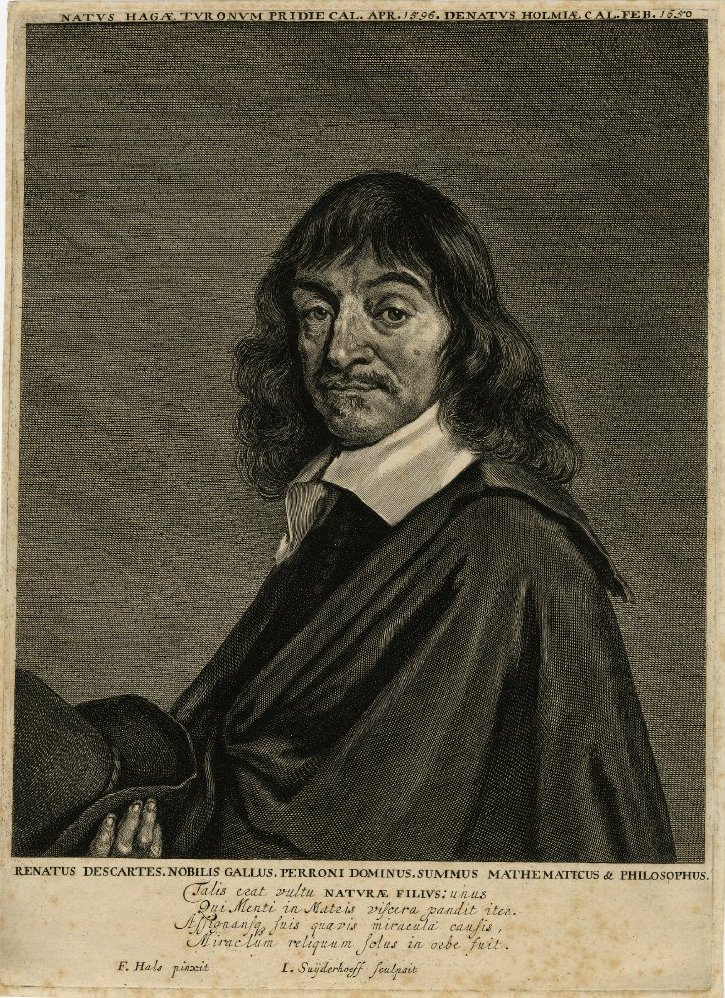
\includegraphics[width = 4cm]{figures/Descartes}
\caption{Portrait of René Descartes}
\label{fig: Descartes}
\end{center}
\end{figure}


Rationalism, in contrast to empiricism, holds the view that knowledge is created mainly by reasoning. In one of the foundational works of modern science, "Le Discours de la Méthode (1637)"  \footnote{The full title of this famous essay is "Discourse on the Method of Rightly Conducting One's Reason and of Seeking Truth" \citep{Descartes-DiscourseMethodRightly-1673}}, René Descartes famously observed: 

\begin{quote}
Good sense is, of all things among men, the most equally distributed; for every one thinks himself so abundantly provided with it, that those even who are the most difficult to satisfy in everything else, do not usually desire a larger measure of this quality than they already possess.\footnote{ These words of one of the founding fathers of what we today consider Science are often read and cited as a sarcastic observation of human vanity. However, if one continues reading, it becomes clear that Descartes may, after all, have been serious about his faith in human rationality. He goes on to state: ``
And in this it is not likely that all are mistaken the conviction is rather to be held as testifying that the power of judging aright and of distinguishing truth from error, which is properly what is called good sense or reason, is by nature equal in all men; and that the diversity of our opinions, consequently, does not arise from some being endowed with a larger share of reason than others, but solely from this, that we conduct our thoughts along different ways, and do not fix our attention on the same objects. ''}
\end{quote}

Rationalists differ though in how exactly knowledge is created by reasoning. Clearly, one can only think if one has some things to think about to start with. Some philosophers have stressed experience as providing these starting points, while others have maintained that there are some innate concepts or truths that we can know without reference to the material world. In either case, a type of reasoning that is natural to rationalism is deductive reasoning

\paragraph{Deductive reasoning}\marginnote{Deductive reasoning = conclude from the general to the specific.} A deduction is when one concludes from the general to the specific. Example: all people from Frankfurt like applewine, I am from Frankfurt, therefore I like applewine. An important difference to inductive reasoning is that, if assumptions are correct, conclusions made by deduction are necessarily correct.


\section{The basic science stance}

In the previous section, we have learned about two fundamentally different thoughts about how knowledge is created (empiricism and rationalism), and we have learned about two types of reasoning (induction and deduction). An attentive reader has probably already drawn a conclusion: in some way, science combines these two views. 

Before we come to that, let me define the basic assumptions that underlie the scientific method:

\begin{itemize}
\item There is a material reality, and we can observe it
\item The material reality follows certain general laws. We can discover the nature of these laws (scientific theory), and we can do this objectively, meaning that everyone sharing the same basic principles (the scientific method) will agree eventually
\item Discovery happens by (a limited number of) empirical observations (empiricism) and reasoning (rationalism), which are combined in the scientific method. 
\end{itemize}


\section{The scientific method and its history}\label{sec: scientific method}

\marginnote{A wider account of the different views on the scientific method on wikipedia \href{https://en.wikipedia.org/wiki/History_of_scientific_method}{here}}


The basic science stance defined in the previous chapter summarizes the basic assumptions of science, but it does not yet tell us how science works in bringing together empiricism and rationalism. 
\subsection{Aristotle's view on the scientific method in his Posterior Analytics}


One of the first\marginnote{Aristotle's six standard works on logic are summarized in the Organon. His view on the scientific method are spread around this work, but the main part is in the the ``Posterior Analytics'', (Latin: Analytica Posteriora).}, certainly one of the best-known explanations of the scientific method is Aristotle's inductive-deductive method (Fig.~\ref{fig: InductiveDeductiveAristotle}). The idea depicted in the figure is the following 

\begin{figure}[]
\begin{center}
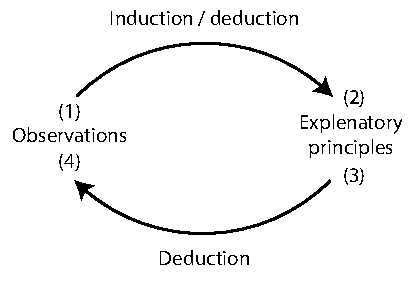
\includegraphics[width = 4cm]{figures/InductiveDeductiveAristotle.pdf}
\caption{Aristotles inductive-deductive model of the scientific method.}
\label{fig: InductiveDeductiveAristotle}
\end{center}
\end{figure}

\begin{enumerate}
\item You make an observation
\item Infer general principles from the observation
\item Infer consequences of these principles
\item Check them against observation
\end{enumerate}

Repeating the cycles of this chain lead to knowledge. 

This basic idea has not changed enormously in the next 2000 years. However, philosophers and scientists have developed different opinions about how the processes of generating explanatory principles and testing them work exactly. A particularly controversial topic has been the extent to which induction plays a role in this cycle. 

Aristotle suggests towards the end of the Posterior Analytics that, at first, explanatory principles arise through induction

\begin{quote}
    Thus it is clear that we must get to know the primary premises by induction; for the method by which even sense-perception implants the universal is inductive. 
\end{quote}

However, he is clearly uncomfortable with the inductive element in this and goes on to say that about the premises created by induction

\begin{quote}
[...] it follows that there will be no scientific knowledge of the primary premises, and since except intuition nothing can be truer than scientific knowledge, it will be intuition that apprehends the primary premises. 
\end{quote}

How this intuition works to create our first premises remains then a bit unclear - but you should read Aristotle yourself, maybe you can make more sense of it than me. 

\subsection{Popper and the scientific method}

We take a 2000yr leap and go the the arguably most influential interpreter of the scientific method in the 20th century - Karl Popper. Popper developed the what we can think of as the current orthodox interpretation of how science works. You may not like it, but due to his influence you will have to face the situation that many people take his views as eternal truths that are set in stone. 


\begin{figure}[]
\begin{center}
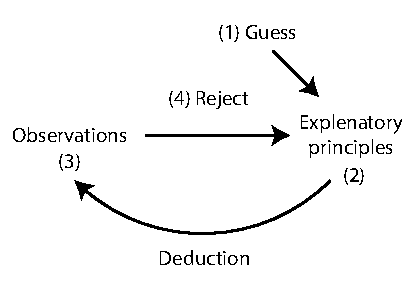
\includegraphics[width = 4cm]{figures/HypotheticoDeductivePopper.pdf}
\caption{Popper's hypothetico-deductive model of the scientific method}
\label{fig: InductiveDeductiveAristotle}
\end{center}
\end{figure}

\paragraph{Hypothetico-deductive method}\marginnote{Popper: you cannot prove a theory, you can only reject it!} In essence, Popper too a radical step to remove induction completely from the equation. According to popper, the essence of science is not to produce new theories, but to have a method to reject them. We don't care how new theories arise: they may be guessed, they may be induced, this is not part of the scientific method. The methods starts once we have a theory - if we a theory is there, we look at the predictions of this theory (deduction), we can test it against observation and see whether the theory is compatible with it (deduction), and if not, we can conclude that the theory is wrong (deduction). Through this construction, science consists only of logically clean deductions. Here a summary of this method 

\begin{enumerate}
\item Form / guess a hypothesis about a phenomenon in nature
\item Derive predictions from hypothesis
\item Test predictions against observation
\item Draw conclusions about the validity of the hypothesis
\end{enumerate}

It follows from Popper that ``you cannot prove a theory, you can only reject'' - hence, avoid using the word proof in scientific articles - many people care deeply about popper, and they will react strongly to it!


\subsection{Multiple working hypothesis}

Popper is the mainstream, but there have been other suggestions about how science works of should work. A counterpoint to Popper's idea of rejection is the idea of multiple working hypothesis. The basic principle is simple - instead of trying to reject an idea, one can work with alternative theories. With time, evidence typically moving to favor one of them. \citet{Platt-StrongInferenceCertain-1964} tracks the history of this idea to an influential essay of the Geologist T. C. Chamberlin, who recommended working with multiple hypothesis to avoid as the best way to avoid “parental affection” (T. C. Chamberlin 1890, Science.

\subsection{Kuhn and variations of the scientific method}

The argument for multiple working hypothesis is a fist example of an argument that brings in the social aspect of how science works - the problem that Chamberlin has with the idea of Popper (he formulated his view before Popper of course) is not that Popper's method wouldn't work in principle, but that in practice, researchers may be hesitant to reject ideas, because they like them to be true. 

A more modern position that goes in a similar direction are the ideas of Thomas Kuhn: in his seminal work ``the structure of scientific revolutions'', Kuhn posits that sciences works within within certain assumptions. In a normal science phase, we may apply Popper's idea to test and improve these assumptions, but we would not reject the basic premises even if there is evidence against them, unless a better theory emerges (revolutionary phase). The phases of science as a according to Kuhn are thus:

\begin{itemize}
\item Pre-paradigm phase – no consensus about a certain phenomenon, incomplete theories
\item Normal science – dominant paradigm emerged, progress in small steps within, but no questioning of paradigm, problems accumulate
\item Revolutionary science – paradigms redefined
\end{itemize}

There is probably a good deal of truth in this observation - in the history of science, there are many examples of the fact that an old theory is only rejected if a better theory is on offer. 

\section{Summary: the principles of science}

Bringing these different theories together, I think it's important not to interpret Aristotle, Popper, Chamberlin or Kuhn as opposing each other - I would simply say that they highlight different aspects of the scientific method as it is applied in practice. 

Popper offers arguably the most pure account of a logically consistent way to use empirical arguments to deductively reject a scientific explanation. However, Chamberlin and Kuhn, however, tell us something about the social rules and necessities that affect scientists and therefore the scientific process. There are many more philosophers worth reading: Francis Bacon, Descartes, Hume, Wittgenstein, Russel, Lakatos - in the larger picture, those are neither right nor wrong, but they simple highlight different aspects of science that as a multi-facetal system of thinking, people and institutions. 

In the hear of all that, however, remains the idea of creating ``near-certain'' knowledge by combining rational thinking with empirical observations.

\vspace{1cm}
\begin{mdframed}
    
\textbf{Repetition of central concepts in this chapter:} 

\begin{itemize*}
  \item Science is based on empiricism and rationalism
  \item Philosophers have tried to remove as far as possible the inductive element out of the scientific method, stressing the deductive parts of science
  \item Popper's scientific method is the orthodox view, but there are other views that stress the aspects of multiple hypothesis of the "social" aspect of the scientific endeavor. 
\end{itemize*}

\end{mdframed}


\chapter{The scientific literature}

Science today is highly specialized. Most basic questions have long been solved. You may think of the scientific enterprise as a "house of knowledge", where one story is built on the next. This is often expressed by a famous quote by Isaac Newton 

\begin{quote}
If I have seen further it is by standing on the shoulders of Giants.
\end{quote}

Regardless of whether the quote was meant as it is interpreted today \footnote{Brian Gottesman notes \href{http://mentalfloss.com/article/24520/6-things-you-should-know-about-isaac-newton}{here}: "Sir Isaac's most famous quotation may well have been an exercise in sarcastic, spiteful anger. In February 1676 Newton wrote to Hooke "if I have seen further it is by standing on the shoulders of Giants." Often taken as a sign of Newton's great humility, this famed quote was almost certainly intended as an insult to Hooke, who was hunchbacked and may have suffered from a form of dwarfism."
}, the fact remains that scientists today are hardly explorers that go far on unmarked territory. 


Before you start a new research project on a particular topic, you should find out what has already been done to a) understand better what you are doing b) avoid doing something that has already been done. 


\section{Finding relevant literature}

How to search for relevant literature depends on the your field, but basically there are three main databases

\begin{itemize}
\item Google scholar 
\item ISI web of knowledge (proprietory, slow, but most "official")
\item Scopus (proprietory, competitor to ISI)
\end{itemize}

All of them work fine, with slightly different interface, search options, advantages and disadvantages. More details in the lecture notes. 

\section{Organizing your literature}

Also the answer to how to organize your literature is pleasingly short - people have created specialized software for this purpose. These reference managers work great, so use them! They will allow you to search in your papers for keywords, names, or anything else, link your pdfs, and they will also couple with your word processing software (MS Word, Open Office, LaTeX). 

\marginnote{See our lab on working with a reference manager \href{https://github.com/florianhartig/ResearchSkills/tree/master/Labs/LiteratureResearch}{here}}

The only question is which of the available programs work best for you. A general recommendation is difficult, as the choice depends next to your personal preferences also on you operating system and your word processing software. You'll find a lot of hints on the internet though, and I also give some short hints on the linked page to the right. 

\section{Citation rules}

Given\marginnote{High-profile cases of "faulty" citations include the former German Minister of Defense Karl-Theodor zu Guttenberg as well as the the former German Federal Minister of Education and Research, Annette Schavan} the amount of PhD titles that have recently been revoked from prominent public figures for not correctly citing the literature in the PhD theses (a charitable expression for outright plagiarism in some cases), it seems a good idea to make sure that everyone is aware of a basic rule in science:

\begin{quote}
If you use the ideas of another person in your work, you need to cite them!
\end{quote}

There are different types of citations:

\begin{itemize}
\item Reference: It is like that (Smith, 2001), or „Smith (2001) expresses the opinion that ...“
\item Quotation: „It is because it is” (Smith, 2001, p.23)
\item Personal communication “Frogs are green (S. Smith, personal communcation)”
\end{itemize}

Taking larger passages / ideas from a source without making this clear is plagiarism. Changing only some words will make it obvious that deliberate intention was involved. Naming the source alone doesn’t make it better when you design the presentation in a way that credit is wrongly attributed to you. By and large, the rules dictated by common sense and honesty apply!

\paragraph{Citation Signals} Citations can be modified by citation signals. An example is the signal ``but'', as in ``It is like it is (but see Adams, 2009)”. These signals are meant to clarify the meaning of a citation, e.g. as supportive, related, or even contradicting the statement made in the main work. Citation signals are therefore crucial, and wrong use can also constitute misconduct! (a few of the high-profile cases with politicians turned around a cf. that was inserted although it should be a direct citation). A list of explanations of the different signals is provided \href{http://en.wikipedia.org/wiki/Citation_signal}{here}. Some of the most important are:

\paragraph{You should read the papers you cite} A recurrent problem, both in student's assignments and in the academic literature, is that papers are cited too broadly or wrongly. \citet{-Causecorrelationconjecture-2015} gives an account of that. \citet{Greenberg-Howcitationdistortions-2009} examine citation networks of papers that are miss-cited. The bottomline is: 1) sure you read the papers that you cite. 2) cite specifically, e.g. by noting in a short sentence for what you cite a paper or what they found, instead of writing only (see also Smith, 2001). 

\vspace{1cm}
\begin{mdframed}
    
\textbf{Repetition of central concepts in this chapter:} 

\begin{itemize*}
  \item You find literature through literature databases
  \item Use a reference manager to organize your literature
  \item Read the papers you cite, cite them correctly for what they say, and don't forget to mention all sources that you use!
\end{itemize*}

\end{mdframed}


\chapter{Questions, data and valid conclusions}

\begin{quote}
For to be possessed of a vigorous mind is not enough; the prime requisite is rightly to apply it. The greatest minds, as they are capable of the highest excellences, are open likewise to the greatest aberrations; and those who travel very slowly may yet make far greater progress, provided they keep always to the straight road, than those who, while they run, forsake it. (Descartes, Le Discours de la Méthode, 1637) 
\end{quote}


If you start a new research project, the first thing to decide on is your question. From that, you develop a hypotheses and experimental procedures to test it and so on. It cannot be stressed enough that the choice of the question is probably the single most important decision in a scientific project. It determines 

\begin{itemize}
\item what you do for the next year / 5yrs / decade
\item whether you identify with your work or not
\item if you can succeed
\item whether anyone cares or not
\end{itemize}


\section{What makes a good scientific questions?}

There have been tons of comments on what makes a good question. If you listen to advice nobel price winners, they often tell you: don't listen to the opinions of the others, do your own thing. This may have become true for them, but certainly not everyone that avoids the mainstream becomes successful. The sad truth may be: it's hard to know in advance what question will make you famous.

That being said, I think it is quite easy to give a few minimum requirements for a good question. 


\paragraph{It has to be new!} A basic requirement is that your question is new, or, as we say in science: novel! Note there may be different levels of new

\begin{itemize}
\item Probably thought of, but not done before (no one bothered)
\item Thought of, but couldn’t be done (because methods lacking)
\item Done, but wrongly (correct previous results)
\item Not thought of before (really new)
\end{itemize}

Obviously, the last item would be the most desirable form of novelty. In any case - check the literature, make sure you understand to which extent your study is different from previous studies

\paragraph{It has to be exciting / relevant!} Your question should be relevant to you, to your community, to society. 

\paragraph{It needs to be a valid scientific question!} We will discuss validity in more detail in the next chaper, but roughly, what is meant by that is: is the question logically consistent, and can we hope to generate a valid answer to it?


\begin{figure}[]
\begin{center}
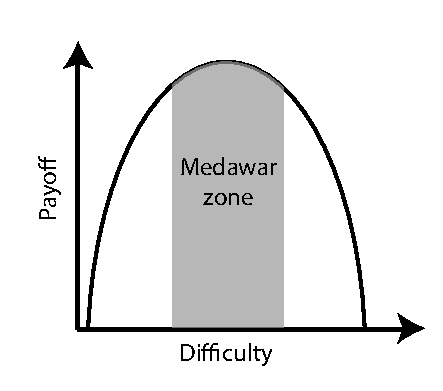
\includegraphics[width = 5cm]{figures/MedawarZone}
\caption{The Medawar zone is an illustration of the sweet spot between too trivial and too difficult questions. The term was coined in \citet{Loehle-guidetoincreased-1990}, in honor of Sir Peter Medawar, who gave a verbal description of this zone in his book `` The Art of the Soluble'' \citep{Medawar-artsoluble-1967}.}
\label{fig: MedawarZone}
\end{center}
\end{figure}

\paragraph{Risks and benefits should balance} In all that, however, you should also make sure that risks and benefits balance - there may be great questions like ``a general cure of cancer'' - it's new, exciting and a valid scientific question. However, if you would try to find an answer in a MSc thesis, you would be set up for failure. Try to find questions that 

\begin{itemize}
\item Don’t test things when the answer is clear
\item To avoid this, don’t pose the question to widely
\item Is a negative result nontrivial? If you can’t show the thing that you expected, is the result still interesting?
\end{itemize}

Great questions\marginnote{If you want to aim really high, you can read the essay ``Ten Simple Rules to Win a Nobel Prize'' by \citep{Roberts-TenSimpleRules-2015}} are also to test a common belief that was not tested before, or question something which was considered established knowledge. 

\section{Experimental design and validity}

Assuming we have a question of interest and novelty, that seems to be worth pursuing - how can we make sure that we set up a valid scientific procedure to answer it?


A framework that allows us to classify the things that can go wrong when we try to apply the scientific method as defined in chapter~\ref{sec: scientific method} is the concept of validity \citep[][]{Shadish-Experimentalandquasi-2002}. The application of these terms is more common in the social science / economics that in natural sciences, but the issues are universal, and for discussing and checking problems I find it useful to have a classification. 

\subsection{Constrcuct validity and bias}

The\marginnote{Construct validity = is what we measure well defined and corresponds to what we mean.} first problem that may appear when we try to test a theory are problems of construct validity. Basically, construct validity means: is what we measure well defined and corresponds to what we mean? Does it correlate with measures it should correlate with (convergent validity)? Is it unrelated to measures it should not correlate with (discriminant validity)?

\paragraph{Construct validity of proxy variables} In "hard sciences" such as physics this is often not so much a concern, but the more we go to complex or social systems, the more likely it is that we measure variables that are proxies for concepts rather than a physical quantity. Examples are "intelligence", "biodiversity", "competition", "light climate". In all these cases, there is probably room for interpretation how to define and measure the concept exactly. It is very advisable to think about his hard, because it can have a strong effect on results. 

\paragraph{Bias} A part of construct validity that is important in either case are potential biases. Biases can appear through instrumental errors, but frequently also through observer bias. More on that in the lecture. 

% TODO \citep{Ransohoff-Biasasthreat-2005}

\subsection{Internal validity}

Internal validity\marginnote{ Internal validity = correlation is not causation} is concerned with the question whether a causal effect can be demonstrated within the experiment / system under study. The basic problem is that correlation does not prove causation. As a an example - if we find that trees have started to grow taller in the last 50 years, and we find that atmospheric carbon dioxide concentration have risen in the same time, we can still not be sure that the CO2 is the causal factor for tree growth. 

Inferences\marginnote{Inferences are said to possess internal validity if a causal relation between two variables is properly demonstrated. } are said to possess internal validity if a causal relation between two variables is properly demonstrated. A more detailed description on this in the \href{https://github.com/florianhartig/ResearchSkills/raw/master/Labs/Statistics/Script/EssentialStatistics.pdf}{accompanying statistics script}, section on experimental design.


\subsection{Statistical validity}

Statistical validity is concerned with the question if an effect has been demonstrated with sufficient statistical (probabilistic certainty). 

Threats to statistical validity are wrong statistical assumptions, but also explicit and implicit biases through malpractices that are known as multiple testing, researcher’s degrees of freedom, low power,P-value fishing / hacking. A more detailed description on this in the \href{https://github.com/florianhartig/ResearchSkills/raw/master/Labs/Statistics/Script/EssentialStatistics.pdf}{accompanying statistics script}. 

\subsection{External validity}

External validity\marginnote{External validity = do extrapolations hold} asks the question: Does our inference about correlations, or cause-effect relationships hold outside the empirical observations available to use. In other word - can we generalize our study, and if so, to what extent. 

The problem with external validity is that it's hard to demonstrate - if we have measured a plot in a particular location, we cannot be sure a priori how representative it is. In practice, it is a matter of experience and common sense to establish the domain on which your results are valid. Nevertheless, this is a very important task, because it is of course crucial for the results of a study to know how generalization they are. 

\vspace{1cm}

\begin{mdframed}
    
\textbf{Checklist validity}%\\[0.4cm]

Before everything else, make sure the question is well defined. I recommend writing it down to avoid ambiguity. Now, check validity of:

    \begin{itemize}
      \item Construct validity
      \begin{itemize}
        \item Do the variables that you can measure match your question?
        \item What could be sources and extend of errors in your measurement (stochastic, systematic), think also about observer bias etc.
      \end{itemize}
      
      \item Internal validity
      \begin{itemize}
        \item What are potential confound or interacting variables?
        \item How are you planning to control / randomize / measure them? Remember, if you can control is better than measure.
        \item Are you sure about the direction of the causality?
      \end{itemize}     
       
      \item Statistical validity
      \begin{itemize}
        \item How will you analyze your data?
        \item What is the sample size that you need (power)?
        \item Are the problems with the independence of your data? How can you minimize those problems (pseudo-replication, blocked design, ...)
      \end{itemize} 
         
      \item External validity
      \begin{itemize}
        \item What generalization are you planning to make from this study?
        \item What are threads to these generalizations / what could be different in other sites
        \item Is there anything in your design that you can change to allow better generalizations?
      \end{itemize}   
    \end{itemize}

\end{mdframed}


\section{Planning and analysis of experiments} 

Assuming that you have a good question, and that you have checked that you have validity of answering it, how do you perform the measurements and how do you analyze them? A detailed description on all this is in the \href{https://github.com/florianhartig/ResearchSkills/raw/master/Labs/Statistics/Script/EssentialStatistics.pdf}{statistics script} accompanying these lecture notes. I highly recommend reading it. I therefore provide here only bullet points of the things that are absolutely crucial to know. 


\subsection{Planning and experimental design}

If you have considered internal validity, you should already know which variables you need to consider. A more detailed discussion on the choice of variables to maintain internal validity (confounding effects) is in the statistics script. 

As a next step, you will have to decide how you vary the value of those variables (if you have control), and how many observations (replicates) you need. Again, this is discussed in more detail in the statistics script, section on experimental design.

Apart\marginnote{Simulate your analysis before going into the field!} from that, I thin the most important tip for planning an experiment is: play it though! What I mean by that is: simulate how you take your data (for real with a pilot study, or make up some data), analyze it, and see if the results of this analysis correspond, in principle, to what you want to know. In most cases, you will notice that the way you were taking data is not optimal for the statistical analysis, that the analysis you do with your data does not answer what you want to know, or something alike. If you notice that before your experiment, it's easy to fix. If you notice it it afterwards, it isn't. 

\subsection{Analysis}

See chapter "inferential statistics" in the \href{https://github.com/florianhartig/ResearchSkills/raw/master/Labs/Statistics/Script/EssentialStatistics.pdf}{statistics script} accompanying these lecture notes.


\subsection{Visualization}

See chapter "descriptive statistics and visualization" \href{https://github.com/florianhartig/ResearchSkills/raw/master/Labs/Statistics/Script/EssentialStatistics.pdf}{statistics script} accompanying these lecture notes.


\vspace{1cm}
\begin{mdframed}
    
\textbf{Repetition of central concepts in this chapter:} 

\begin{itemize*}
  \item A good scientific question is novel and important, and you should expect to be able to give a valid answer with a acceptable risk of failure
  \item Validity is a classification scheme of problems that can arise when trying to give an answer to a scientific question. See the validity checklist.
  \item You should plan your experiment thoroughly. Part of good planning is that you play the complete process trough before taking the data, including the analysis.
\end{itemize*}

\end{mdframed}



\chapter{Principles and channels of communication}

If you have made a scientific discovery, or at least a little bit of scientific progress, you probably want to let the world know about it. Hence, you need to be able to communicate.

\section{Principles of communication}

Thinking about communication requires a fundamental change in our attitude - up to now, we have dealt with ourselves, and how to generate knowledge. It was all about finding out the truth. Communication, however, is different. It is not necessarily about saying things right - it is about saying the right things. 

What I mean by that is that the end of communication is not to say things as correct or truthful as they are - the thing that counts is that they are received as correct and truthful as possible in your audience. Good communication therefore requires adjustment, according to your audience. For any form of communication, you should therefore ask yourself the following basic questions:


\begin{enumerate}
\item Rule1: Who is my audience?
\item Rule2: What is my main message?
\end{enumerate}

and adjust your words, level of detail and complexity, and jokes accordingly. A few general hints, however, can be given:



\paragraph{Clarity} Science is about getting this right - the main goal of (scientific) communication is therefore clarity and logic. 

\paragraph{KISS} People in science\marginnote{The KISS principle - Keep it short and simple!}, however, are also busy - this means you need to communicate efficiently. Both goals are served well by the KISS principle - Keep it short and simple! However, don't forget Einstein: “as simple as possible, but not simpler”.\footnote{This is also reflected in the following remark by Niels Bohr “Never express yourself more clearly than you are able to think.”}

\paragraph{Jargon} To reach the goals outlined above, Jargon can be a good and a bad thing. It can make communication more efficient, but you have to be careful - this is only the case if you and the recipient have the same jargon. Jargon used in a wrong way is worse than no jargon.






\section{Communication channels}



\subsection{Books and articles}

The most important form of scientific communication is arguably the written word, in form of books and articles. A longer description on how a scientific article is structured is given in the following chapter. 


\subsection{Oral presentations}

The probably second most important channel are presentations. That is, in the perception and attention of many people. Especially young scientists are very concerned with presentations, because they are often used to determine marks of projects and so on. But also for older scientists, presentations are crucial, for example in job interviews. It is therefore important to have some skill in this type of communication \citep[see, e.g. the tips of][]{Kelleher-Tenguidelineseffective-2011}. More material on poster presentations on our lab on oral presentation. 

Personally, though, I am not sure how important presentations still are in shaping scientific thinking. It seems to me that the scientific debate and thinking relies more strongly on written media, either journal articles, or nowadays blogs, discussion forums and so on. These media are able to reach a much wider audience than a typical conference talk that is visited by maybe 50 people that may see another 30 talks on the same day. All this is not to say that oral presentations are not important - they may be crucial for getting a job. I just think that once you have it, science is driven by different media. 

\subsection{Poster presentation}

A similar case are poster presentations - on many conferences, poster presentations are offered for participants that don't give a talk. Poster presentations are a great opportunity to meet people and start discussing about your work, but I don't think they rank nearly as high in terms of importance than journal articles. More material on poster presentations on our lab on posters. 


\subsection{Blogs, social media, and such}

Blogs, social media and similar outlets have become more important in recent years. A collection of things that are worth checking out is provided in our lab on social media.



\section{Arguments and logical fallacies}

In his article ``Sounder thinking through clearer writing'', \citet{Woodford-Sounderthinkingthrough-1967} 


\begin{itemize}
\item False dilemma - if we want everything to be completely correct, we can stop doing science!
\item False equivalence - no model is completely perfect, therefore there is no difference between using model A and B
\item Strawman - proving an argument wrong that is similar, but not identical to that of the opponent - A: Diversity can increase ecosystem function. B: my opponent suggests that     diversity increases human well-being. But this is clearly wrong. Imaging a world where we have no HIV virus. Now, if I introduce the virus, we have more diversity. But human well-being is clearly lower!
\end{itemize}




\vspace{1cm}
\begin{mdframed}
    
\textbf{Repetition of central concepts in this chapter:} 

\begin{itemize*}
  \item Good communication means not saying the right thing, but that your recipient understands what you want him/her to understand - the road to hell is paved with good intentions!
  \item You should know the different communication channels of science. The most important ones are the oral presentation and the scientific paper (next chapter)
  \item Be aware of rhetoric structures and logical fallacies. As a good scientist, you must be able to see through them!
\end{itemize*}

\end{mdframed}



\chapter{Scientific writing}


Writing is an essential skill for an academic, as for many other professions. \marginnote{The importance of the written word does not seem to change at all in the modern world. The art of writing, similar to public speaking, seems to be one of the stable skills that one can think of.} Despite its central role, however, few master it well. Writing is a subtle art. You can read some advice, but to become a skilled and effective writer requires a long process of observation, practice and reflection: read widely, and think about why some writers appeal to you more. Look critically over your own writing, and think about the things that you can improve. The rest of this section is intended to help you start this journey. 

\section{Some basic writing advice}

\paragraph{Start writing early}\marginnote{Please, follow this point in your thesis - if you don't it leads foreseeable into disaster!} Writing structures your thinking, and you will find flaws in your logic that you didn't see before. "The time to begin writing an article is when you have finished it to your satisfaction. By that time you begin to clearly and logically perceive what it is that you really want to say." (Mark Twain)

\paragraph{Know your audience}\marginnote{\citet{Gopen-ScienceOfScientific-1990} state "it matters only whether a large majority of the reading audience accurately perceives what the author had in mind".} Who is going to read what you write?  You need to adjust your text to the knowledge and background of your audience. 


\paragraph{Know what you want to say, and make a selection}\marginnote{"If you don't know where you are going,you'll end up someplace else" (Yogi Berra). } Sounds trivial, but in my experience it isn't. Before spending hours on writing the wrong text, try to explain a friend in 5-10 min the essential points of piece, and note the structure. If you fail with this, think again about your story. Also remember: Writing a good paper is not about telling everything you know or have done about a topic -- it is about telling a story and selecting the relevant details. 

\paragraph{Mindset} Make your goal, above all, clarity of thought and expression, and impervious logic of your argument. Read \citet{Woodford-Sounderthinkingthrough-1967}.

\paragraph{Respect conventions}\marginnote{For example, the default scientific article is divided into a title, abstract, introduction, materials and methods, results and discussion. Within these structural elements there are further recognizable patterns. Maintaining this structure makes it easier to understanding of the article's messages \citep{Gopen-ScienceOfScientific-1990,Tischler-Scientificwritingbooklet-1978}} Readers, particularly experienced readers, are familiar with writing conventions expect to find arguments, sections and statements in particular positions and structures. If the writer respects these structural standards the readability is greatly improved. 


\paragraph{Modesty} Think of a scientific text as a piece of craftsmanship, like a chair. What is expected of you is to produce a simple chair that respects the usual standards (e.g. four legs), and that is, above all, solid. You are not expected to add fancy ornamentation that might be used by an ingenious master craftsmen, and produce a entire set of furniture that would suffice to fit out a house. If you could do the later, you would gain admiration and praise, but when trying, you will nearly certainly fail to even produce the very thing you were asked for - a simple, solid chair. Bottomline: stay modest in what you want to achieve, but stay ambitions in how you achieve it!


\paragraph{Style} Writing is difficult. Good writing is incredibly hard. If you think writing is no problem for you, you probably haven't even realized the extent of your writing problems. Read the following section twice!


\section{Style}


\subsection{Sentence Structure}

\begin{quote}
The battle for good writing is won sentence by sentence! A good sentence is: short, has the subject and verb together, has an active verb, has the points of emphasis at the beginning and end, and moves the reader along from a familiar launch point at the start to the new information at the end. (Brian McGill, on the blog Dynamic Ecology)
\end{quote}



\subsection{Paragraph structure}

A paragraph is a logical unit of text. 

The first sentence provides the topic of the paragraph. The last sentence should, ideally, provide a closing 



\href{http://www.economist.com/styleguide/introduction}{http://www.economist.com/styleguide/introduction}

%\href{http://www.nature.com/authors/author_resources/how_write.html}{http://www.nature.com/authors/author_resources/how_write.html}



\subsection{Logic}


\subsection{Clarity}

Keep it simple. \footnote{Mark Twain is famous for his effective writing. A tip from him: "As to the Adjective: when in doubt, strike it out."}



\section{The structure of a scientific article}   
% general strucutre
On the largest unit of discourse the research paper comprises a title, abstract, keywords, and an introduction, methods, results and discussion section (and where required appendices). 
This structure somewhat forces the writer to repeat the story of the paper over and over again. In the end  it should be told roughly $3\frac{3}{4}$ times -- once with the title, once with the abstract, a quarter in the introduction, half in the discussion/ conclusion, and again once with the whole article.

%hourglass structure
Another structural element concerning the general layout is the "hourglass structure". This means the writer should start off with general information, becoming then more and more specific and completing with a link to the general again. Yet, it only applies to the abstract and (more flexibly) to the whole article.\\
 
%individual sections/elements
%title
\paragraph{Title}
Zooming in to the next smaller unit of discourse we start off with the title. %\marginnote{\large{\textsc{the title}}}
Its main purpose is to interest potential readers since 97~\%  of them only read the title. To keep them reading the title should signal the topic. A good tip is to make it precise and informative with a hint at the findings -- it should reflect the main message of the article's story.\\

%keywords
\paragraph{Keywords}
The author is asked to list some keywords, %\marginnote{\large{\textsc{the keywords}}}
which are usually located right below the abstract. These terms allow people to find the article when searching with ISI web of knowledge. Yet, since Google scans whole documents the keywords are probably not as important as they used to be. Nevertheless, a good strategy is to choose keywords complementary to title and abstract, e.g. for important technical terms that you
did not want to include in the abstract nor title.\\

%abstract
\paragraph{Abstract}
The abstract %\marginnote{\large{\textsc{the abstract}}} 
is the second time you will tell your story; in fact it can be considered as a mini paper. It starts off by setting the scene with a very short and general introduction. This usually links to the second part: Raise the problem. You can emphasize the research question by indicator words like "however". Here you tell why your work is necessary.\marginnote{To make sure you follow this structure it may be helpful to copy a template into your manuscript.} Third, you briefly delineate your approach. The fourth subsection serves to state the results. Finally, you present your conclusions and discuss the broader significance.\\

%introduction
\paragraph{Introduction}
The first main section of the article is the introduction. %\marginnote{\large{\textsc{the introduction}}}
It comprises four parts: Start of with one or two paragraphs outlining the broad topic and what work has been done before.\marginnote{Go from the general\\ ...to the specific\\ ...but not back to the general.} Here you usually cite a lot of literature showing that you know the current state of knowledge concerning the topic of your study.
Use another one or two paragraphs to explain the problem, i.e. the gap of knowledge. Here, you may sell your idea and why the knowledge gap needs to be filled.
Then, delineate your approach in one paragraph: What are your methods; what are the data you used?\marginnote{Make use of indicator words to clarify the role of the individual paragraph: however; problem/ challenge; here we used; we applied; we asked; we tested.}
Finally, you may list your specific research questions. This subsection does not need to be clearly separated from the approach subsection. It should however, provide a link to the result sections by outlining the work flow of the analysis.\\

%methods
\paragraph{Methods}
In the methods section %\marginnote{\large{\textsc{the methods}}}
the reader learns precisely what has been done. Even though details may be important this section should not take up too many words, since the total amount for the paper is usually fairly limited by the publishing journal\marginnote{Keyword is repdoucibility.}. You will have to make a selection here; technical information, which is necessary to replicate the study (Software version, etc.) can be moved to an (online) appendix. This may even increase the readability. If helpful the methods section may also be divided in subsections such as study area, data, statistical analysis/ model, analysis, etc. Another helpful tip is to add figures. They can greatly enhance the ability of the reader to understand your approach. Furthermore, if there were any problems with your methods, do not discuss them here -- use the discussion for that.\\

%results
\paragraph{Results}
Now that you have explained your methods and the course of analysis, present your results in the next section.%\marginnote{\large{\textsc{the results}}}
Here you will have to make a selection once again. The results you show need to be relevant to your story, and need to match the specific research questions you lay out in the abstract and more importantly at the end of the introduction. To clarify your findings it is helpful to use figures.\marginnote{Facts are better conveyed short and simple!}
Remember the most important aspect about this section: Your results need to be presented as neutral facts. Do only state what is obvious, but leave speculation for the discussion. You may however give an interpretation and cross links if they are obvious.\\

%discussion/conclusion
\paragraph{Discussion/ Conclusion}
Finally, we need to wrap up the article.%\marginnote{\large{\textsc{the discussion/ conclusions}}} 
The discussion/ conclusion section comes commonly at last but with extensive functionality. It contains a summary of the main findings. Remember here, many of your readers only read this section (and the title)\marginnote{Move from the specific\\ ...to the general.}. It is common to summarize by restating the problem, significance and the methods in the beginning. Secondly, this section is the platform to discuss the results, speculate about reasons and theories and for the connection to other literature.\marginnote{Only discuss the limitations that question/limit the credibility of your results.}
As was mentioned before, this section is the place where you may tell the reader about the limitations of your approach and possibly the reasons why the main findings are still credible. However, rather establish the domain under which your results are valid; do not question your approach in general. Finally, the reader expects you to provide conclusions, recommendations, applications and questions for further research.\\

\section{Showcase: A commented paper}

\begin{center}
	\huge{Fancy analysis supports hypothesis\marginnote{Try to capture the questions, methods, and main results of your study in the title, if possible} X as the main cause high species diversity in tropical forests} \\ 
	\vspace{0.3em}
	\large{Florian Hartig and Severin Hauenstein}\\
	\vspace{0.3em}
	\small{\textit{Department of Biometry and Environmental System Analysis, University of Freiburg, 79106 Freiburg, Germany}}\\
	\vspace{1em}
	\large{\today}\\
	\vspace{2em}
	\textbf{Abstract}\\ \marginnote{Remember: the abstract is a mini-paper}
\end{center}
\begin{quote}
Tropical forests are some of the most species-rich ecosystems\marginnote{First words set the scene} of the world.
The reason for this, \textbf{however}, is still widely debated\marginnote{Raise the problem. Indicator word: however}. Hypotheses range from processes related to productivity over environmental stability to the historical changes in geography.
\textbf{Here}\marginnote{Introduce your approach. Indicator word: here}, we contrasted these different hypotheses by using data from ... together with ... (fancy new method).
\textbf{We find that}\marginnote{State your results. Indicator word: We find, our results are ...} hypothesis X seems to be significantly better supported by our data
than all alternatives we tested. Specifically ... 
\textbf{In conclusion}\marginnote{Give your conclusions and discuss wider significance. Indicator word: in conclusion, ...}, our study supports the hypothesis that species diversity in the
tropics is mainly driven by higher productivity. These results challenge some long held
ideas about geographical stability being the main reason for global diversity
patterns. They also have important practical applications for mitigation of climate
change, as ...\\[0.3cm]
\noindent\textbf{Keywords:} Biodiversity -- Primary production -- Floristic structure ...\\
\end{quote}

\noindent\textbf{Introduction}\\
Tropical forests provide a suitable habitat to a vast variety of species. According to XY (19XX) tropical forests make up fo x \% of the planet's biodiversity.\\
...

Many ecologists have aimed at explaining this phenomena and a large number of hypotheses has been published in recent years (e.g. ABC, 19XX; D\&E, 20XX; FG, 20XX). However, not all of whom have made convincing arguments. To order the state of knowledge validation and comparison of the studies is desperately needed.\\
...

In this short note, we compare a set of pre-selected hypotheses published by ABC (19XX), D\&E (20XX), FG (20XX) and ... and present a validation of the used approaches. For the latter we used X data provided by XYZ (2014)\\
... 

We first test X in order to find the difference in Y. As an alternative approach we choose to look at Z for the purpose of XY. Specifically we are interested in species Y. Furthermore, the validation of the hypotheses will provide information about ...\\
...\\
In the following we briefly outline the concepts of ... and present our validation approach.\\
...

\noindent\textbf{Methods}\\

\noindent\textbf{Results}\\

\noindent\textbf{Discussion}\\
In this study, we used method X to test whether prevalence of A
is associated to factor B. Our main result is that there is a
significant correlation of B with A. This correlation, however, was
only found when factor C was also present.

Our findings support earlier findings of (X, 2005) and (Y, 2002)
who also found a positive correlation between A and B. The fact
that this correlation was only present in samples under conditions
C may also explain previous opposite results such as (ZZ,
2006,2008), as neither of these previous studies controlled for C.
The reason for this positive association and the fact that it is
affected by C is still unknown. We speculate that mechanism R
could be a reason for this. This idea is given further support by
the observation that the correlation between A and B is affected
by C. Such an effect would be expected if R is really the cause of
this Correlation, as R is dependent on C (XAY, 1968).



\section{A list of common writing problems}


\begin{enumerate}[(A)]


\item Strategic writing problems
\begin{enumerate}
	\item Do not make statements that are unnecessary for your argument, but could be questioned. 
	Example: "The two most classic games to simulate the behavior of animals are the Hawk-Dove game and the Prisoner's Dilemma." $\rightarrow$ Others might disagree. Is it really important to be so definite here? Why not say: "Two classic games..."?
	\item Passive/ Active: See the comments in the lecture notes on scientific writing. In general you should write in an active voice, unless  1) Sentence structure C3 takes precedence, or 2) the thing you talk about is impersonal, was done by another person. More details in the lecture notes. In particular, opinions of your own \textsc{should} be active.
	\item Be definite - remember Yoda: There is no try, do it. Phrases like: "we attempted to find whether there is" or "this study aims at" sound weak and defensive. Write "we studied whether ...". Also: "to the best of our knowledge ... " This is a borderline case. You will see this expression in scientific articles, and it's OK to use it. However, it does seem insecure. Better to indicate that you made some effort to find out together with such an expression. 	
	
 

\end{enumerate}

\item Logical problems
\begin{enumerate}
	\item The stated implication does not follow the argument logically. Example: "Because both models follow different pay-off schemes, it is important to know how a simulation model reacts to different settings." $\rightarrow$ Unclear why it is important to know how simulation reacts to different settings if two models are different.
	\item "Micrologic": Logical indicators such as "thus", "hence", "however", "nevertheless" have a clear and distinct meaning. "thus", "hence" indicate an implication. "however", "nevertheless" indicate contradicting statements or evidence to the previous proposition.
\end{enumerate}


\item Style
\begin{enumerate}
	\item Drop redundant words: Any of the following \textbf{words} can be erased: "\textbf{a total of} n subjects", "the simulations were run with the \textbf{exact} same parameter set as before"
	\item Pompous/ pontificating style: If something can be said in simple words, it should be said in simple words, i.e. if the only purpose of a sentence is to "sound scientific", it should not be said at all. Examples: The data \textbf{featured/comprised} a pixel size of 10 (had). We utilized (use).\footnote{Styleguides advice against complicated words such as utilize if there are simpler equivalent alternatives, although others have argued that there is a different between use and utilize - but could you name it? See discussion here \href{http://en.wiktionary.org/wiki/utilise}{here}.} We used the model in an integrated framework to facilitate a holistic forecast" (predicting from the model). Tip: Read \citet{Woodford-Sounderthinkingthrough-1967}.
	\item Topic position/ Stress position not properly occupied: The first part of a sentence should give the context. The last part of the sentence should provide the crucial new information, and should relate to what is further discussed. Tip: Read \citet{Gopen-ScienceOfScientific-1990}.
	\item A paragraph structures the text into topical units. Use them! Each paragraph should introduce its topic in the beginning, and ideally lead to some conclusion or summary at the end. 
	\item Unnecessary adjectives. Mark Twain: "As to the adjective: when in doubt, strike it out." Especially adjectives such as "very", "particularly" are often not necessary. Applies also to larger constructs such as "Evolutionary Game Theory \uline{is an important tool to} investigate(s) ..." -- if you erase the underlined text, the sentence remains fine.
	\item Unclear/ ambiguous expressions: Write as clear and as informative as possible. Avoid ambiguous words like "tends to", "mostly" etc. if you can make a definite statement. Example: "the frequency of cooperators always tends to be zero"  $\rightarrow$ What does that mean? 1) It was always zero or 2) It was zero in 95 \% of the cases or 3) something else.
\end{enumerate}

\item Grammar and spelling

\begin{enumerate}
	\item English commas have different rules than in German and other languages \url{http://www.grammarbook.com/punctuation/commas.asp}
	\item Wrong use of \textbf{which and that} Let's say that we have 10 samples. Compare the two sentences: 1) the samples, which were expose to radiation the day before, were analysed. 2) The samples that were exposed to radiation the day before were analyzed. The important difference is that 1) says all samples were exposed to radiation and then analysed, while 2) implies that not all samples were exposed to radiation, and only those that were were analysed. 1) is called a non-restrictive clause, and 2) is called a restrictive clause. "that" always implies a restrictive meaning. Additional confusion, however, is created by the fact that "which" can in fact be used for both, with a minor modification: if you want to use which restrictive, you have to write 3) The samples which were exposed to radiation the day before were analyzed. Notice that there is a tiny difference to 1) - there is no comma before which. This is the only indicator that allows us to know whether the restrictive or the non-restrictive meaning is implied. Many people are not aware of this difference though. In prose, the distinction may matter little, but for science, my opinion is that clarity goes before style, and I therefore recommend to strictly stay with 1) which for non-restrictive and 2) that for the restrictive meaning.
\end{enumerate}



\end{enumerate}


\section{Examples}

In the following, I highlighted \uline{redundant words} and other problems

\begin{itemize}

\item A \uline{subsequent} ANOVA \uline{analysis} \textbf{enabled a quantification of} the impacts of the varied factors (quantified)

\item There are \uline{a number of records} in the literature \uline{focusing on comparisons} between \uline{sets of }modeling approaches while predicting biomass at plot scale (A number of previous studies has compared modeling approaches to predict biomass at the plot scale)

\item \uline{As such}, the \uline{explicit} findings of our two experiments showed that \uline{a total of} 9 samples ... 

\end{itemize}


\vspace{1cm}
\begin{mdframed}
    
\textbf{Repetition of central concepts in this chapter:} 

\begin{itemize*}
  \item You find literature through literature databases
  \item Use a reference manager to organize your literature
  \item Read the papers you cite, cite them correctly for what they say, and don't forget to mention all sources that you use!
\end{itemize*}

\end{mdframed}

\chapter{A working scientists}

Up to now, we have covered the primary scientific process from deciding on a scientific question, generating valid data and conclusions, and communicating those in writing or through other channels. However, as hinted to in the introduction, science is also a human endeavor, and as such, a professional scientist should also be aware of the norms and codes of the field, as well as the realities of a life in science. The purpose of this chapter is to give a very fast overview on this questions.

\section{Professional ethics and good scientific practice}

The term "good scientific practice" encompass

\citep{Forschungsgemeinschaft-RulesGoodScientific-2013}

\marginnote{The rules of the German Science Foundation (DFG) are available \href{http://www.dfg.de/en/research_funding/principles_dfg_funding/good_scientific_practice/}{here}. Other guidelines for good scientific practice are available \href{https://github.com/florianhartig/ResearchSkills/blob/master/Labs/AcademicSoftSkills/codesOfConduct.md}{here}}


\subsection{Documentation}


There is no clear legal rule about how long data, documentation and samples have to be stored, but most funding organizations require 



\subsection{Honesty}




\marginnote{Simple things like having a good folder structure for each project help a lot. Have a look at our lab on \href{https://github.com/florianhartig/ResearchSkills/tree/master/Labs/ProjectOrganization}{project organization}}


\marginnote{When working with code, specially collaboratively, there is no way around using a version control system. See our lap on version control \href{https://github.com/florianhartig/ResearchSkills/tree/master/Labs/VersionControl}{here}}


\section{Social aspects}

\subsection{Collaborations and teams}

\subsection{Conflicts}

\subsection{Intercultural issues}


\section{Science as a career}



\marginnote{Read the special feature in Nature on the \href{http://www.nature.com/news/specials/phdfuture/index.html}{future of the PhD}}


\vspace{1cm}
\begin{mdframed}
    
\textbf{Repetition of central concepts in this chapter:} 

\begin{itemize*}
  \item You find literature through literature databases
  \item Use a reference manager to organize your literature
  \item Read the papers you cite, cite them correctly for what they say, and don't forget to mention all sources that you use!
\end{itemize*}

\end{mdframed}


\bibliographystyle{/Users/Florian/Home/Bibliography/Databases/bibstyles/elsart-harv-hyperlinks}
\bibliography{/Users/Florian/Home/Bibliography/Databases/flo}

\end{document}
